\chapter{Experimental work and results in mode I}
\label{Chapter3}

\section{Introduction}

This chapter outlines the experimental work to investigate mode I fracture using MMCG specimens using the DIC method. Firstly, the experimental set-up is described in detail. Subsequently, the mode I results are presented, and the energy release rates for mode I MMCG samples are calculated and discussed in relation to existing literature.

\section{Experimental set-up}

The fracture tests were performed using a Landmark Servohydraulic testing machine with a maximum capacity of 100 kN. Figure~\ref{fig:Setup0°} shows the experimental set-up, which includes the Arcan fixture and the optical camera-lens-illumination devices. The Arcan fixture was mounted to the testing machine using standard bolts, with washers inserted between the specimen and the Arcan system to reinforce the attachment points. To facilitate specimen changes between tests, manual controls were employed to elevate the moving part of the testing machine, minimising residual tension between the bolt holes and the Arcan system. Furthermore, before testing, an arbitrary pre-load was applied to the specimen to prevent any clearance or unintended movement of the specimen (which could cause image defocusing). Load and cross-head displacement data were recorded at a frequency of 5 Hz . Additionally, a real-time plot was generated during the test for visualisation.


An Alvium 1800 U-2040m Allied Vision camera and a 60 mm Nikkor lens were used for image grabbing and acquisition. The camera has a resolution of 4512 (H) $\times$ 4512 (V) and a sensor size of type 1.1. The front of the lens was positioned at a working distance of 285 mm with an aperture of f/11 and an exposure time of 60 milliseconds. The cross-head displacement of the testing machine was 0.02mm/s, and the camera had a frequency of 1 Hz (1 fps).
 A green illumination set-up was used to enhance the sensitivity of the sensor. The camera was securely mounted on a tripod to ensure a stable position relative to the specimen's target surface, enabling the capture of consistent images throughout the tests. The frontal face of the specimens was coated with a suitable speckle pattern. A first layer of white paint was added and a cloud of black dots formed a second layer of paint. Figure~\ref{fig:Speckle_DIC} shows an image of the speckle pattern, along with its corresponding image histogram. Additionally, a scale positioned in the surface plane was employed to establish the conversion factor for translating pixels into millimetres.


\begin{figure}[htp]
	\centering
	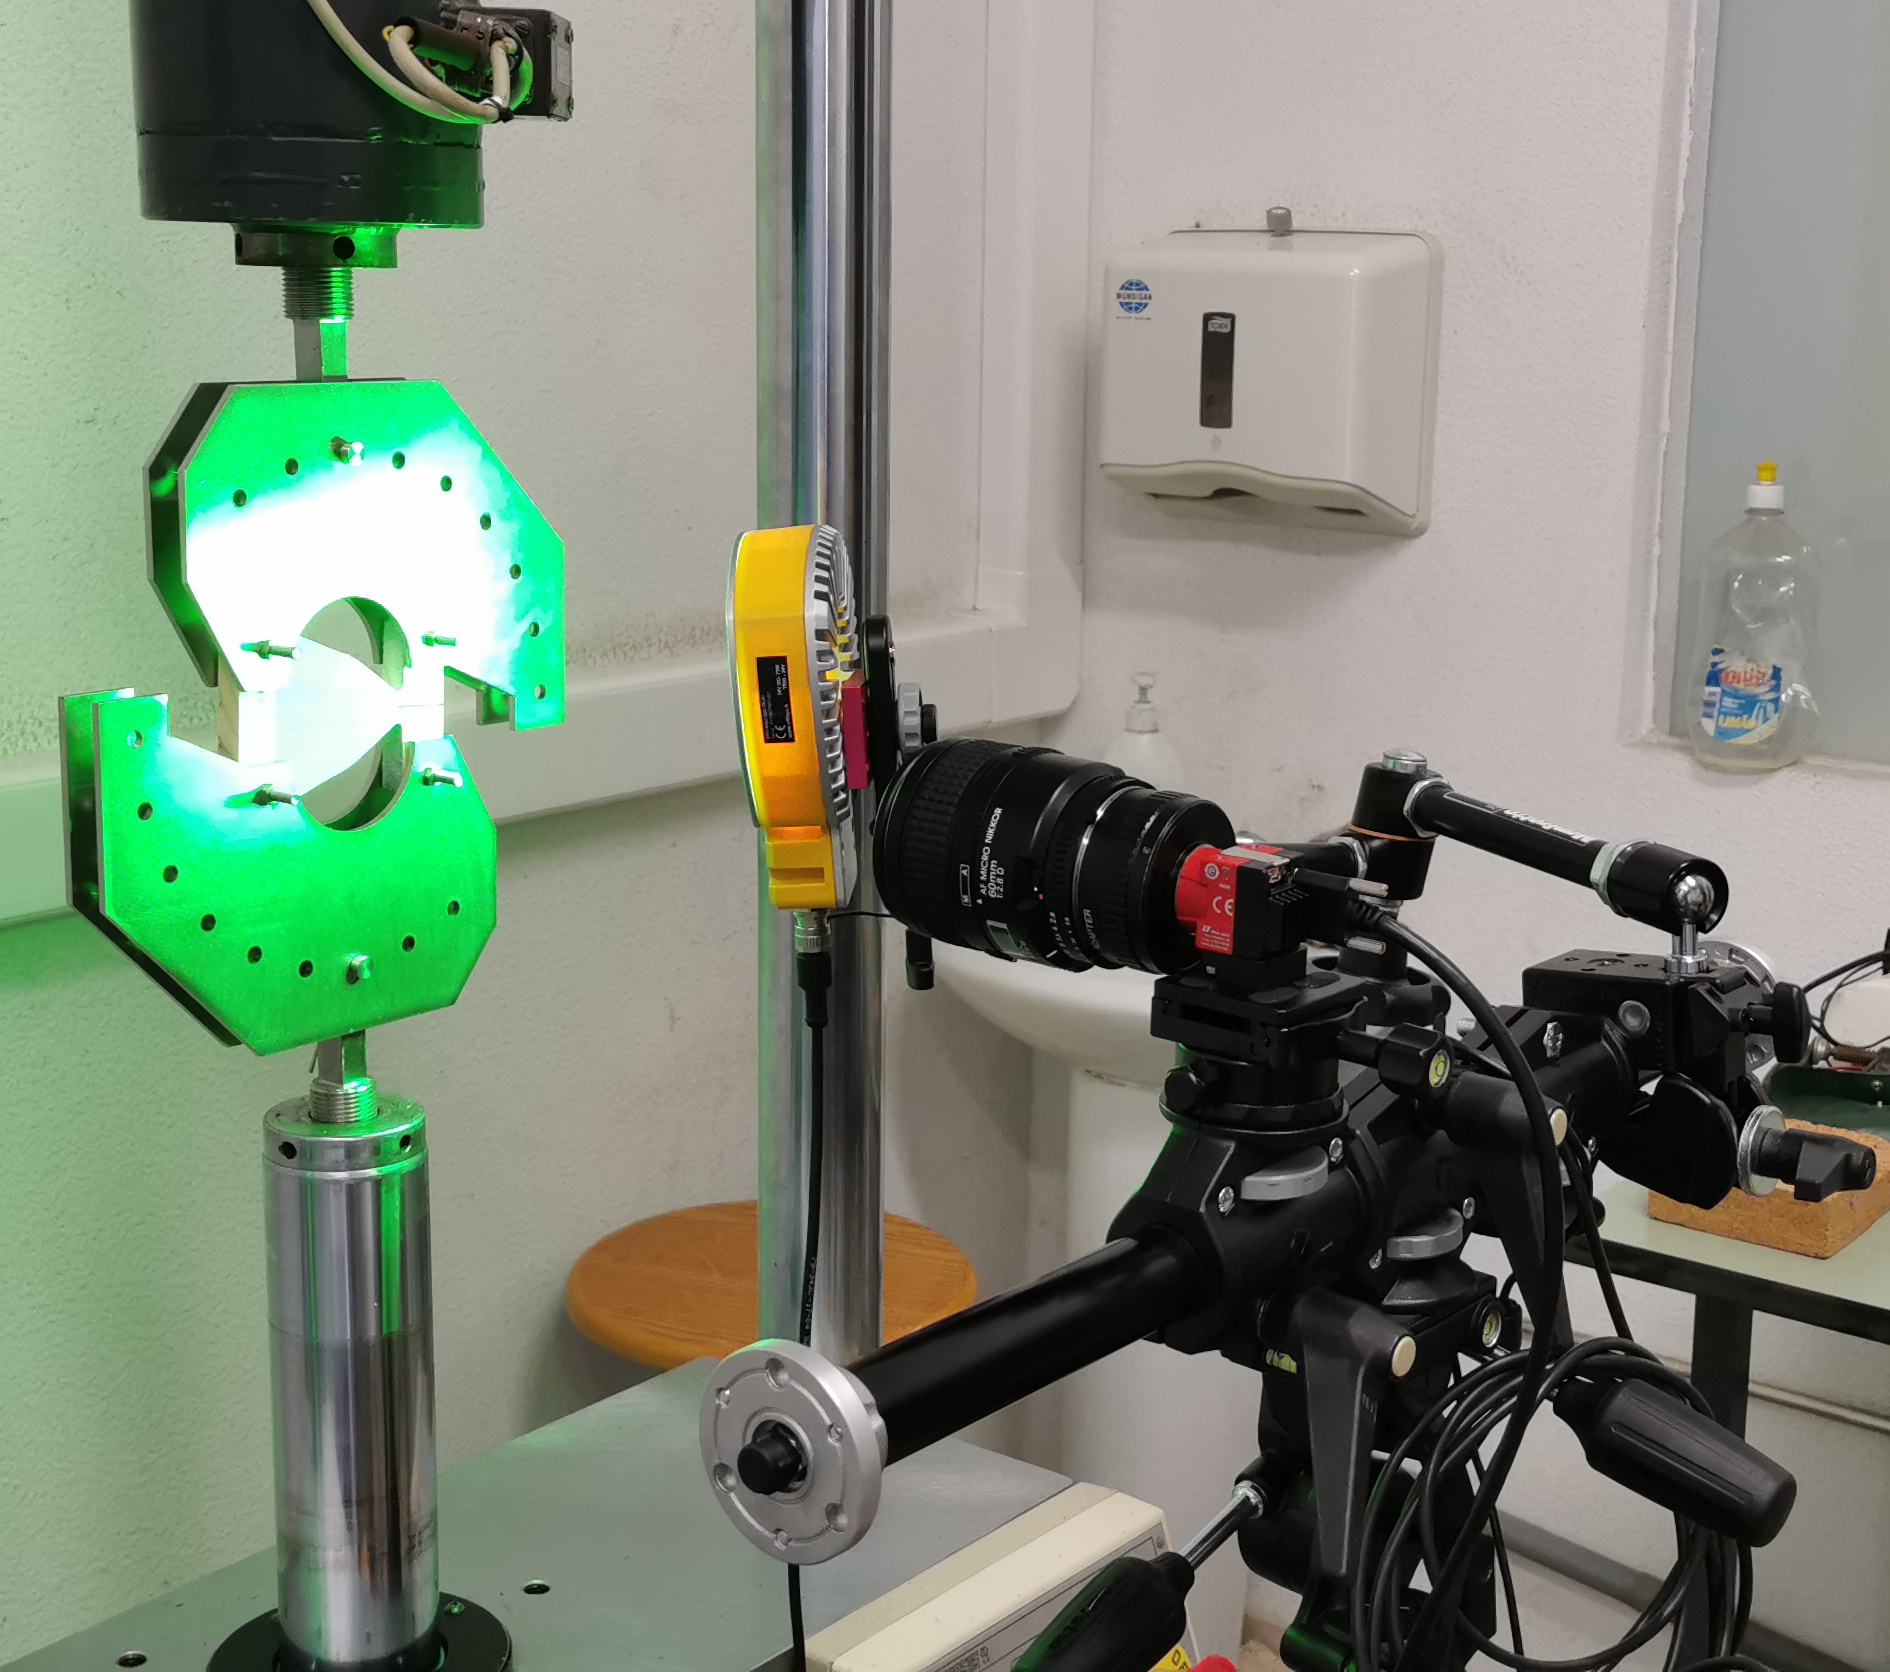
\includegraphics[width=.6\textwidth]{Setup0_crop}
	\caption{Experimental set-up.}
	\label{fig:Setup0°}
\end{figure}


\begin{figure}[htp]
	\centering
	\begin{tabular}{c}
		\includegraphics[width=5cm]{Speckle_DIC} \\
		(a) \\
		\\
		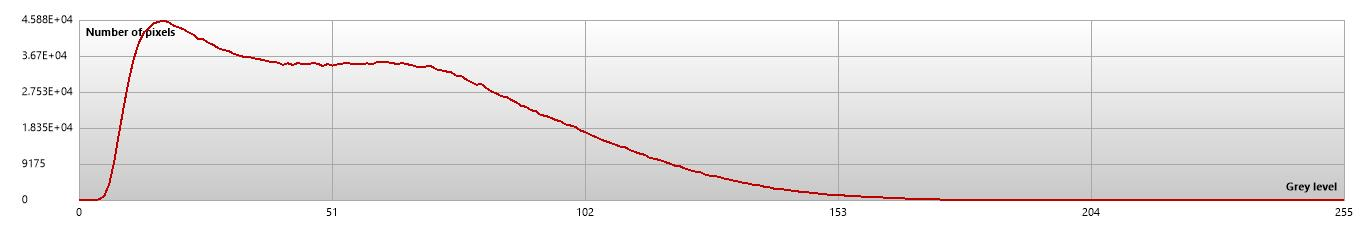
\includegraphics[width=16cm]{histogram} \\
		(b) \\
		\\
	\end{tabular}
	\caption{(a) Speckle pattern typically obtained with DIC; (b) Histogram of the speckle image.}
	\label{fig:Speckle_DIC}
\end{figure}


The selected parameters for the DIC analysis play a crucial role in determining the accuracy and spatial resolution of the measured displacements and reconstructed strain fields \citep{Xavier2012207,PereiraandXavier2018}. Consequently, they are considered fundamental factors. To achieve a trade-off between spatial resolution and accuracy, a parametric analysis was conducted utilizing the Parametric Module of MatchID. The resulting DIC settings are summarized in Table~\ref{tab:MatchID_param}.

The range of values defined in this performance study, including the subset size ($f_s$), subset step, affine and quadratic displacement shape functions, the size of the strain windows, and the order of the polynomial fitting function, is defined by the table \ref{tab:MatchID_param}. It is believed that the pre-selected range of values is reflective of the permissible DIC setup parameter range.

\begin{table}[]
	\centering
	\begin{tabular}{m{.3\textwidth}m{.4\textwidth}}\toprule
		Correlation   Coefficient: & ZNCC \\
		Interpolation order: & Bicubic Splines \\ 
		Transformation order: & Quadratic \\
		Prefiltering: & Gaussian \\
		Progress history: & Spatial \\
		Subset size: & 31 \\
		Step size: & 10 \\
		Strainwindow size: & 5 \\ 
		Virtual Strain Gauge: & 71 pixel \\
		Strain interpolation: & bilinear (Q4) Lagrange polynomials\\
		Strain Convention: & Green-Lagrange \\\bottomrule
	\end{tabular}
	\caption{DIC setting parameters used in the MatchID software for the analyses.}
	\label{tab:MatchID_param}
\end{table}


\section{Results and comparison in mode I}

\subsection{Load-displacement curves}

Normally four distinct parts are observed on a load-displacement curve for Mode I fracture loading:

\begin{itemize}
	\item A small area visible at the beginning of the curve which corresponds to the setting up of the loaded specimen. 
	\item A nearly linear region arises from the elastic loading phase with a static crack front.
	\item The third segment is distinguished by a series of critical force peaks, which signify a distinct crack initiation. The progressive increase in these peaks confirms the crack's stability zone.
	\item Lastly, the final segment entails the material's rupture, which transpires when an ultimate force is applied, marking the instability of the crack.
\end{itemize}

Because of the preload applied at the fixture and specimen adjustments, the raw load and displacements were slightly shifted to reproduce the initial conditions of zero displacements and load at the reference configuration. This extrapolation is possible because the curve has an initial linear regime. All load-displacement curves are summarised in appendix \ref{Appendix1}.


\begin{figure}[htp]
	\begin{minipage}[c]{.46\linewidth}
		\centering
		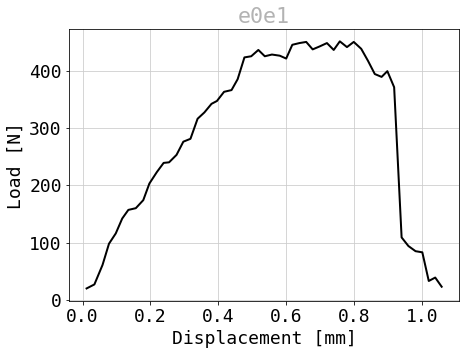
\includegraphics[width=8cm]{P_e0e1}
		\caption{Characteristic load-displacement ($P-\delta$) curve.}
		\label{fig:e0e1_Pdelta}
	\end{minipage}
	\hfill%
	\begin{minipage}[c]{.46\linewidth}
		\centering
		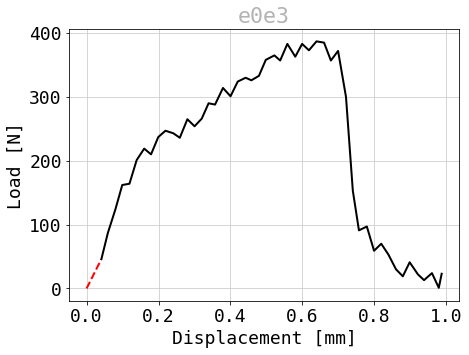
\includegraphics[width=8cm]{P_e0e3}
		\caption{load-displacement ($P-\delta$) curve shifted.}
		\label{fig:e0e5_Pdelta}
	\end{minipage}
\end{figure}


\subsection{Deformation fields}

Typical deformation map ($\epsilon$yy) obtained with the DIC method is shown in Figure \ref{fig:Strain_def}.
During the tests we noticed that the cracks tend to propagate according to the orientation and inclination of the fibres.
In Figure \ref{fig:Strain_def} for specimen e0e1, we assume a small fibre inclination which could explain the crack orientation that we see.

\begin{figure}[htp]
	\centering
	\begin{tabular}{c}
		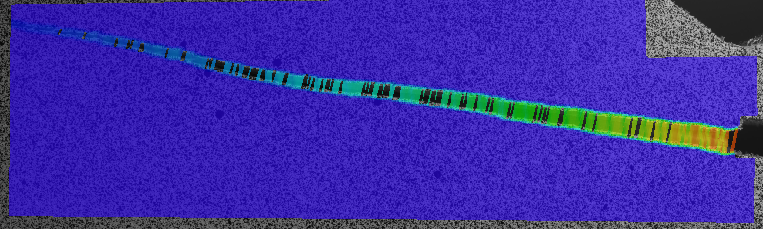
\includegraphics[width=8cm]{e0e1} \\
		e0e1 deformation map \\
		\\
		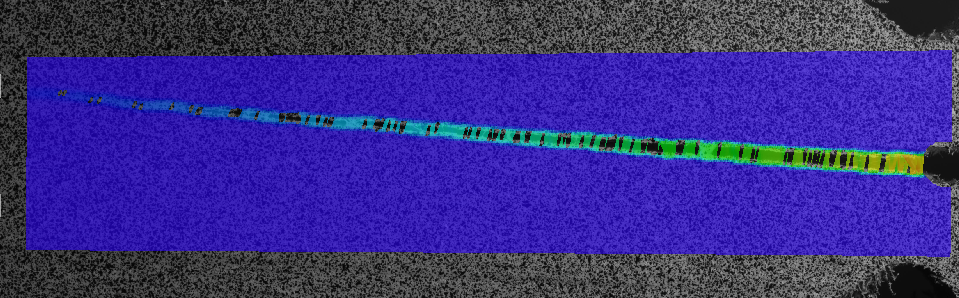
\includegraphics[width=8cm]{e0e2} \\
		e0e2 deformation map \\
		\\
		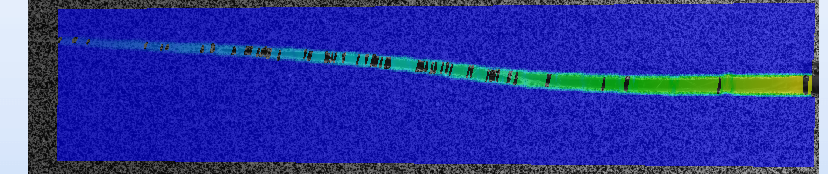
\includegraphics[width=9cm]{e0e3} \\
		e0e3 deformation map \\
	\end{tabular}
	\caption{Typical deformation map ($\epsilon_{yy}$) obtained with DIC.}
	\label{fig:Strain_def}
\end{figure}

Strain maps are used to best locate the position of the crack tip by graphic reading.
Thus, thanks to the deformation maps we are able to obtain the crack length on different stages. It is then possible to check whether method 1 and method 2 are working correctly.
The blue points Figure \ref{fig:fig39} and \ref{fig:fig40} for tests e0e2 and e0e3 are the points read graphically with the deformation maps. We can see that the blue points follow the curves of method 1 correctly, so we can consider that the method is working correctly.
It seems that method 2 is less accurate than method 1, but we'll still use it to obtain G and see what difference a small variation in a(t) will do.

\begin{figure}[htp]
	\begin{minipage}[c]{.46\linewidth}
		\centering
		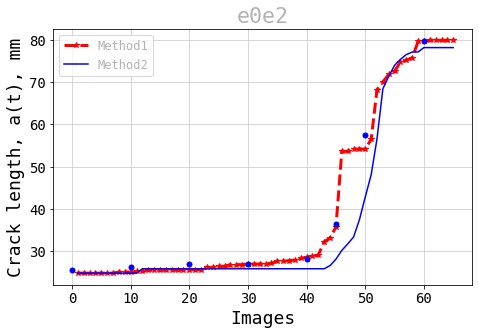
\includegraphics[width=8cm]{e0e2_graphicread}
		\caption{Crack tip by graphic reading e0e2.}
		\label{fig:fig39}
	\end{minipage}
	\hfill%
	\begin{minipage}[c]{.46\linewidth}
		\centering
		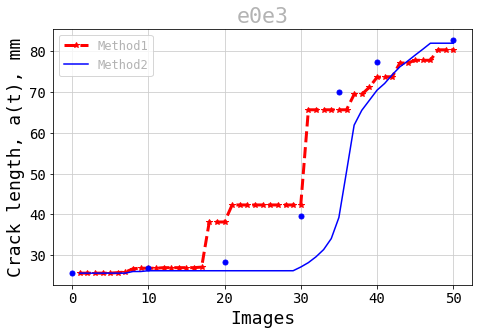
\includegraphics[width=8cm]{e0e3_graphicread}
		\caption{Crack tip by graphic reading e0e3.}
		\label{fig:fig40}
	\end{minipage}
\end{figure}


\subsection{Crack tip opening curves}

The user must select the "CTODpair". In order to provide accurate displacement, the chosen pair of subsets must be as close as possible to the crack tip while yet being sufficiently removed to prevent information loss (if they are positioned inside the crack). Databases are updated using the selected CODpair following this study. Due to the selected CTOD pair being in blue, a plot was produced that displays the CTOD that were used, as seen on Figure \ref{fig:CTOD_example}. In order to demonstrate for each specimen that the COD pair picked could not have been more exact, the plot also compared this curve to the one created using the lower and upper COD pairs.

\begin{figure}[htp]
	\centering
	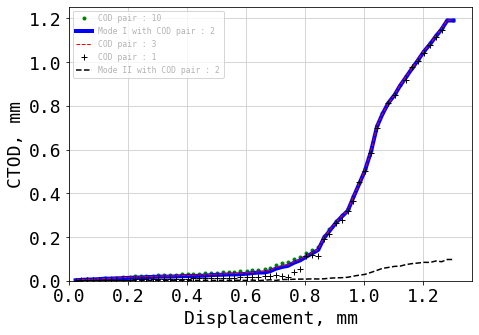
\includegraphics[width=9cm]{CTOD_example}
	\caption{Crack Tip Opening Displacement choice.}
	\label{fig:CTOD_example}
\end{figure}

All the crack opening curves in mode I (displacement of the two lips of the crack) are shown in Figure \ref{fig:COD_modeI}.
We can see two distinct phases in these curves. A first phase in which the force increases with a slight increase of the CTOD and a second phase in which the load decreases with a sharp increase of CTOD. In the first phase, the MMCG specimen resists the force applied by the tensile machine, whereas in the second phase, the crack is already well initiated. There is therefore little resistance for the wood sample, which explains why the force decreases and the CTOD increases significantly.
Only the portion of the curve before the abrupt force P decrease will be used to calculate G. If we use curve e0e6 as an example, we can see that the specimen breaks at a CTOD of around 1.2mm due to an abrupt decline in force.

\begin{figure}[htp]
	\centering
	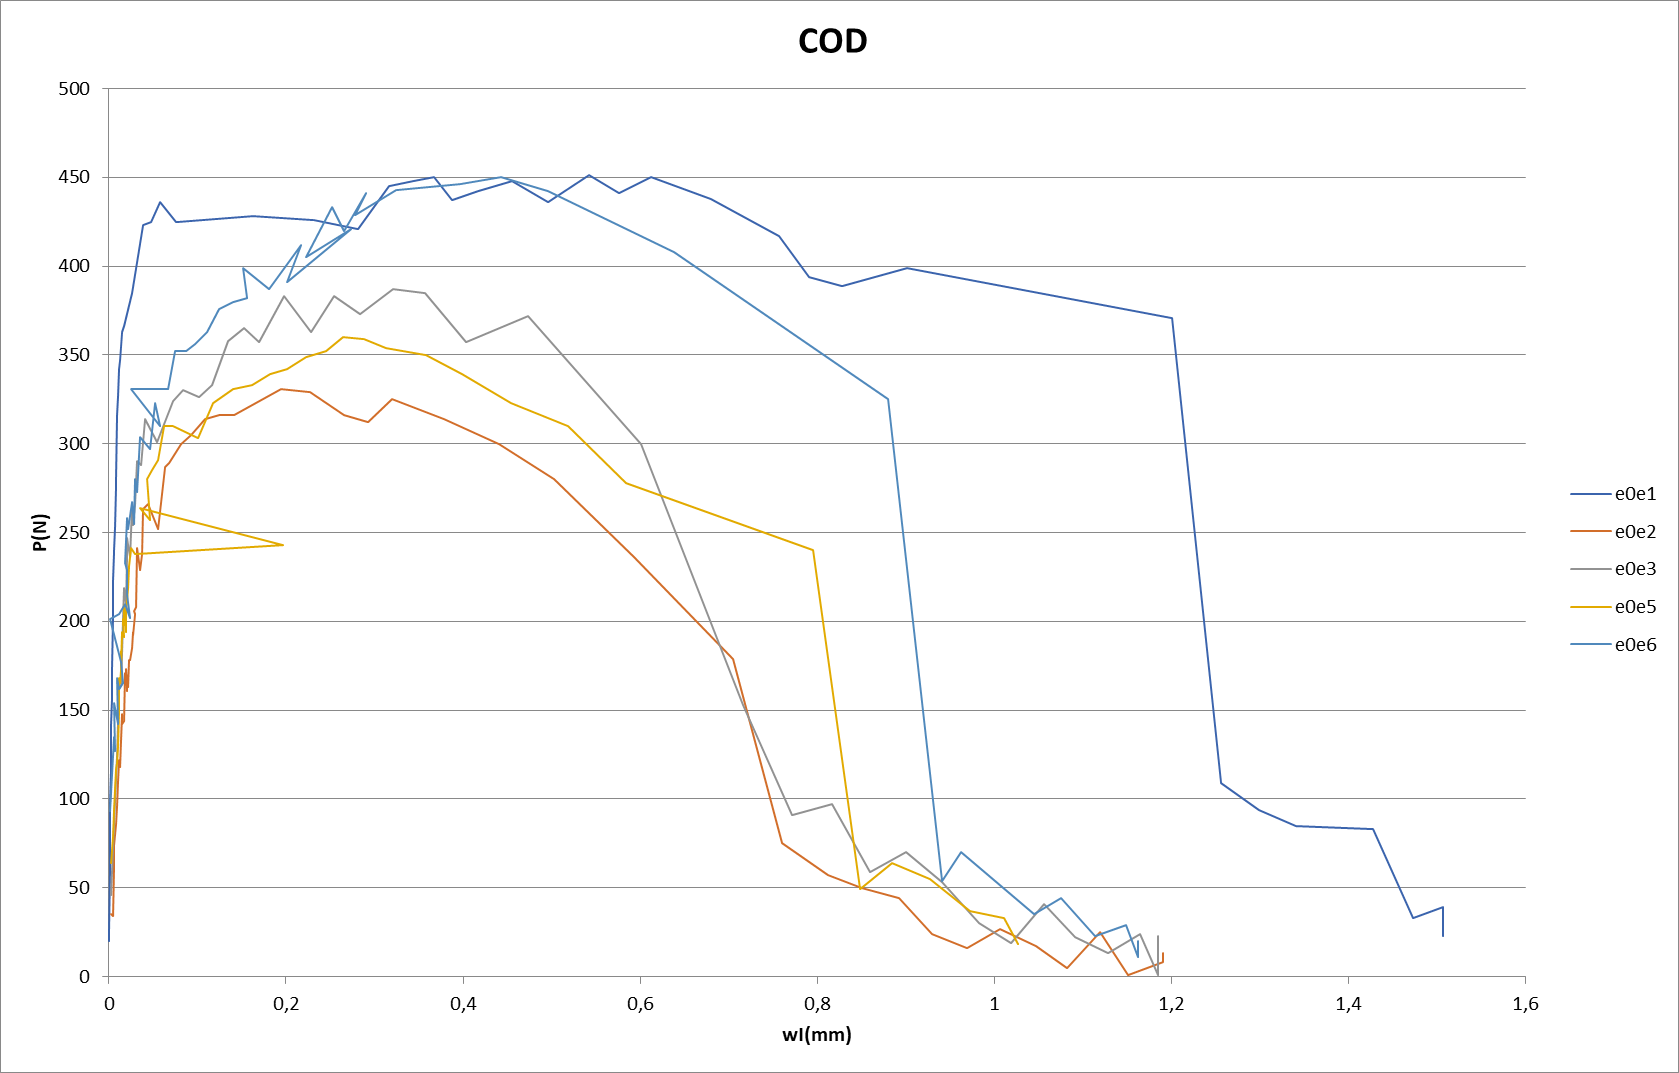
\includegraphics[width=13cm]{COD_modeI}
	\caption{Crack Tip Opening Displacement.}
	\label{fig:COD_modeI}
\end{figure}

\subsection{Crack length curves}

For method 1 by compiling the evolution of a(t) as a function of the images recorded for several alpha values (\ref{fig:Cracklength_modeI_example}), it is possible to get an idea of the alpha value required to obtain the best a(t). Indeed, the alpha parameter must be as small as possible for the evolution of the crack length to be complete. So, for each crack length in the sample, it is possible to eliminate several candidates. In this example \ref{fig:Cracklength_modeI_example}, it is possible to eliminate the use of curves with a(t)<70mm. These alpha values do not allow the entire crack length to be studied. To distinguish between the black and turquoise curves, you can place the position of the crack tip with a red dot on the displacement map. Then for different stages, we can then see which curve corresponds best to the position of the crack tip. Here, the black curve was chosen.

To obtain a(t) using method 2, we need to read $a_1$ and $a_f$ graphically and choose a pair of COD lines that are not damaged by nans values.

\begin{figure}[H]
	\centering
	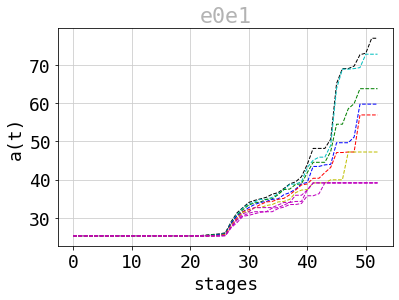
\includegraphics[width=9cm]{Cracklength_modeI_example}
	\caption{Crack length evolution depending on alpha.}
	\label{fig:Cracklength_modeI_example}
\end{figure}

All the crack length curve in function of displacement in mode I are shown in Figure \ref{fig:crack_method1} and \ref{fig:crack_method2}.
With method 1, there are, as expected, different plateaus for the crack length.The crack length increases gradually and continuously before rupture. It is the design of the MMCG specimen that allows the stable propagation of the crack. Indeed, with this specimen, cracks progress slowly until failure occurs at maximum load. In some images, bridges prevent the fracture from propagating linearly. When these bridges break, the crack propagates, involving a new stage. It is interesting to examine all the crack length propagation plots.  The curves are all more or less the same shape, and the crack ends at roughly the same length. What differs is the stage at which the crack begins to propagate. For example, we can see that e0e1 begins its crack propagation at stage 23, whereas e0e2 begins at stage 9 for method 1.
As for method 2, it gives broadly the same curves as the method 1 but the curves are smoother, which is not necessarily a good thing since crack propagation in wood normally works more step by step. Moreover, if we check the Figure \ref{fig:a_e0e1} or Figure \ref{fig:a_e0e2} in the appendix  we can see that the crack length of method 2 is generally lower than that of method 1 for the same stage.

\begin{figure}[htp]
	\centering
	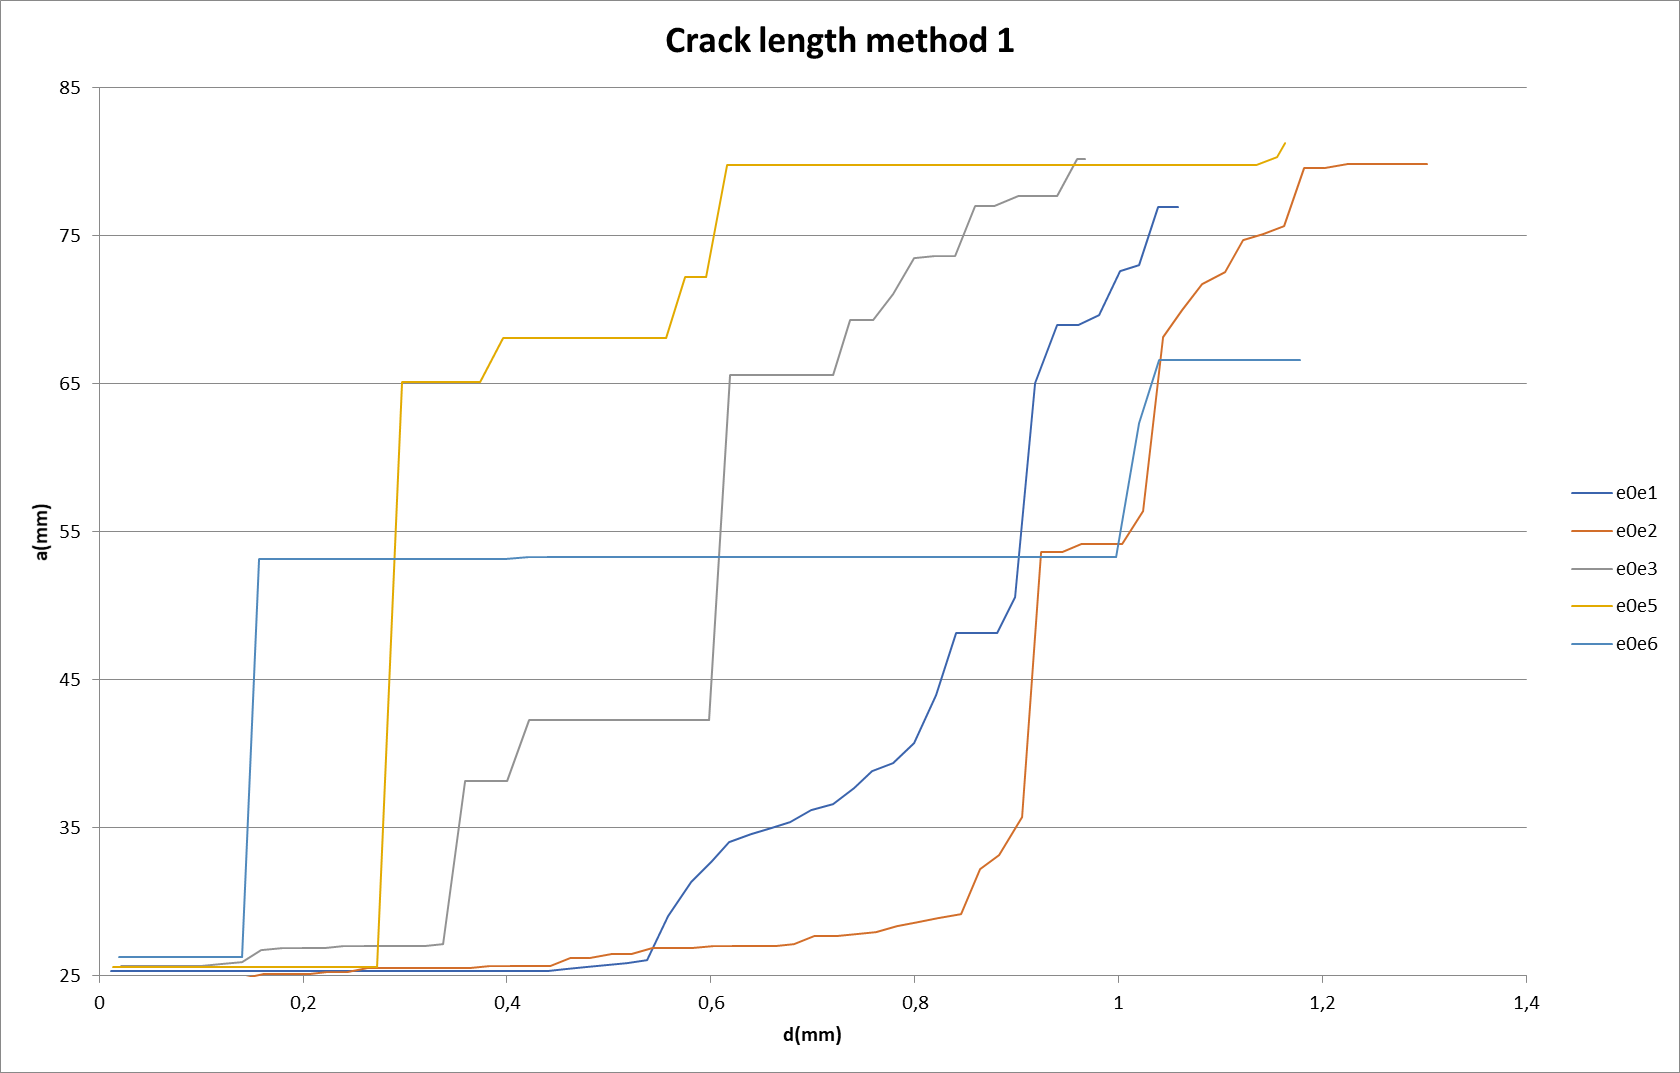
\includegraphics[width=13cm]{crack_method1}
	\caption{Crack length evolution method 1.}
	\label{fig:crack_method1}
\end{figure}

\begin{figure}[htp]
	\centering
	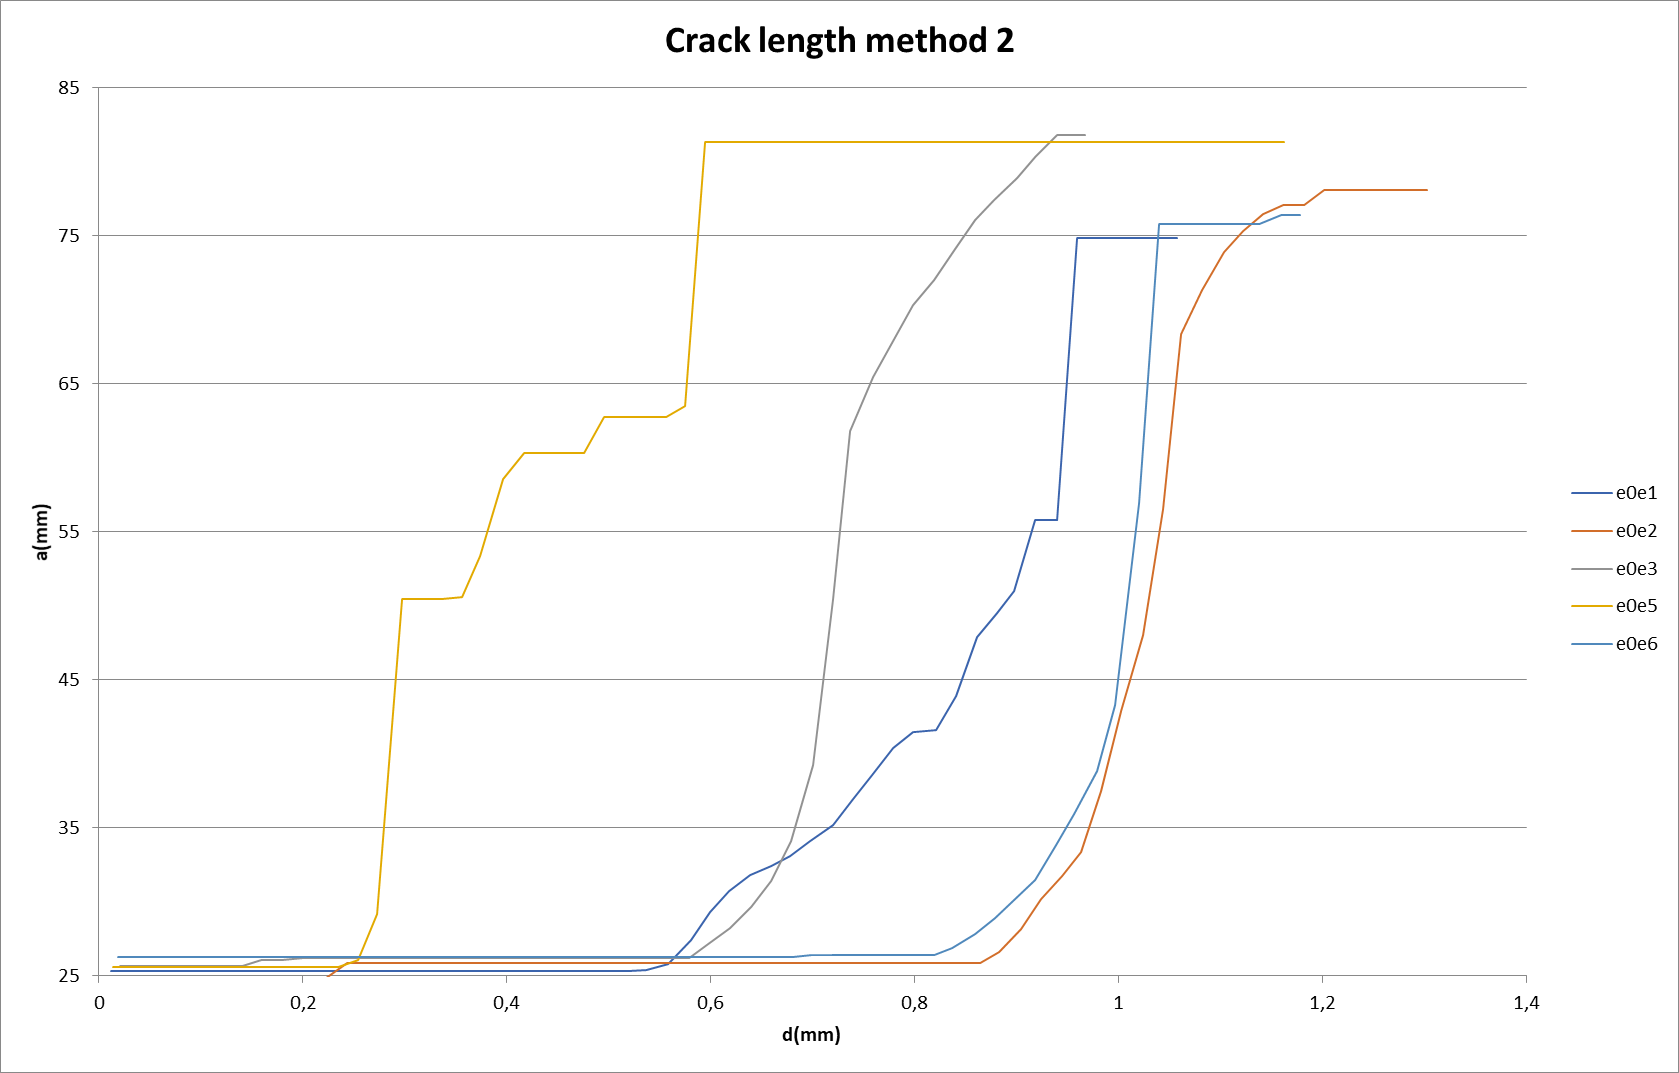
\includegraphics[width=13cm]{crack_method2}
	\caption{Crack length evolution method 2.}
	\label{fig:crack_method2}
\end{figure}

\subsection{Critical energy release rate}

Various methods can be used to calculate the energy release rate. The general formula is explained in \ref{eq:eq125}. However, it is possible to calculate compliance in different ways. One possibility, used by \cite{MALFAIT2021} and \cite{MoutouPitti2008}, is to calculate the $\Delta c$ between the starting point and the point considered for all the critical forces. The critical forces are the forces for which the force decreases at the next stage, meaning crack propagation according to \cite{MoutouPitti2008}. A second possibility is to determine C as an interpolated function as $C(a)=m*a(t)^3+n$ with a(t) the length of the crack.  It is then possible to use the compliance derivate by the crack length. Both were tested to see which would be better and finally G is calculated with $\Delta c$. In fact, the cubic function used did not pass through all the points on the graph of C as a function of a(t) and was therefore very inaccurate. The values of G obtained with this method were of the order of $10^3 J/m2$, which is too high.
The figures \ref{fig:G_method1} and \ref{fig:G_method2} below show G with the 2 methods used to calculate the crack length.
As can be observed, depending on the specimen, different values of a(t) are reached with the maximal energy release rate. For values of a(t) between 33 and 80 mm, method 1 and 2 achieve Gmax, with an apparent tendency for Gmax to be acquired at a(t) about 60 mm with method 1. For method 2, Gmax is obtained for shorter crack lengths. This can be explained by the fact that a(t) is generally smaller for the same stage.

\begin{figure}[htp]
	\centering
	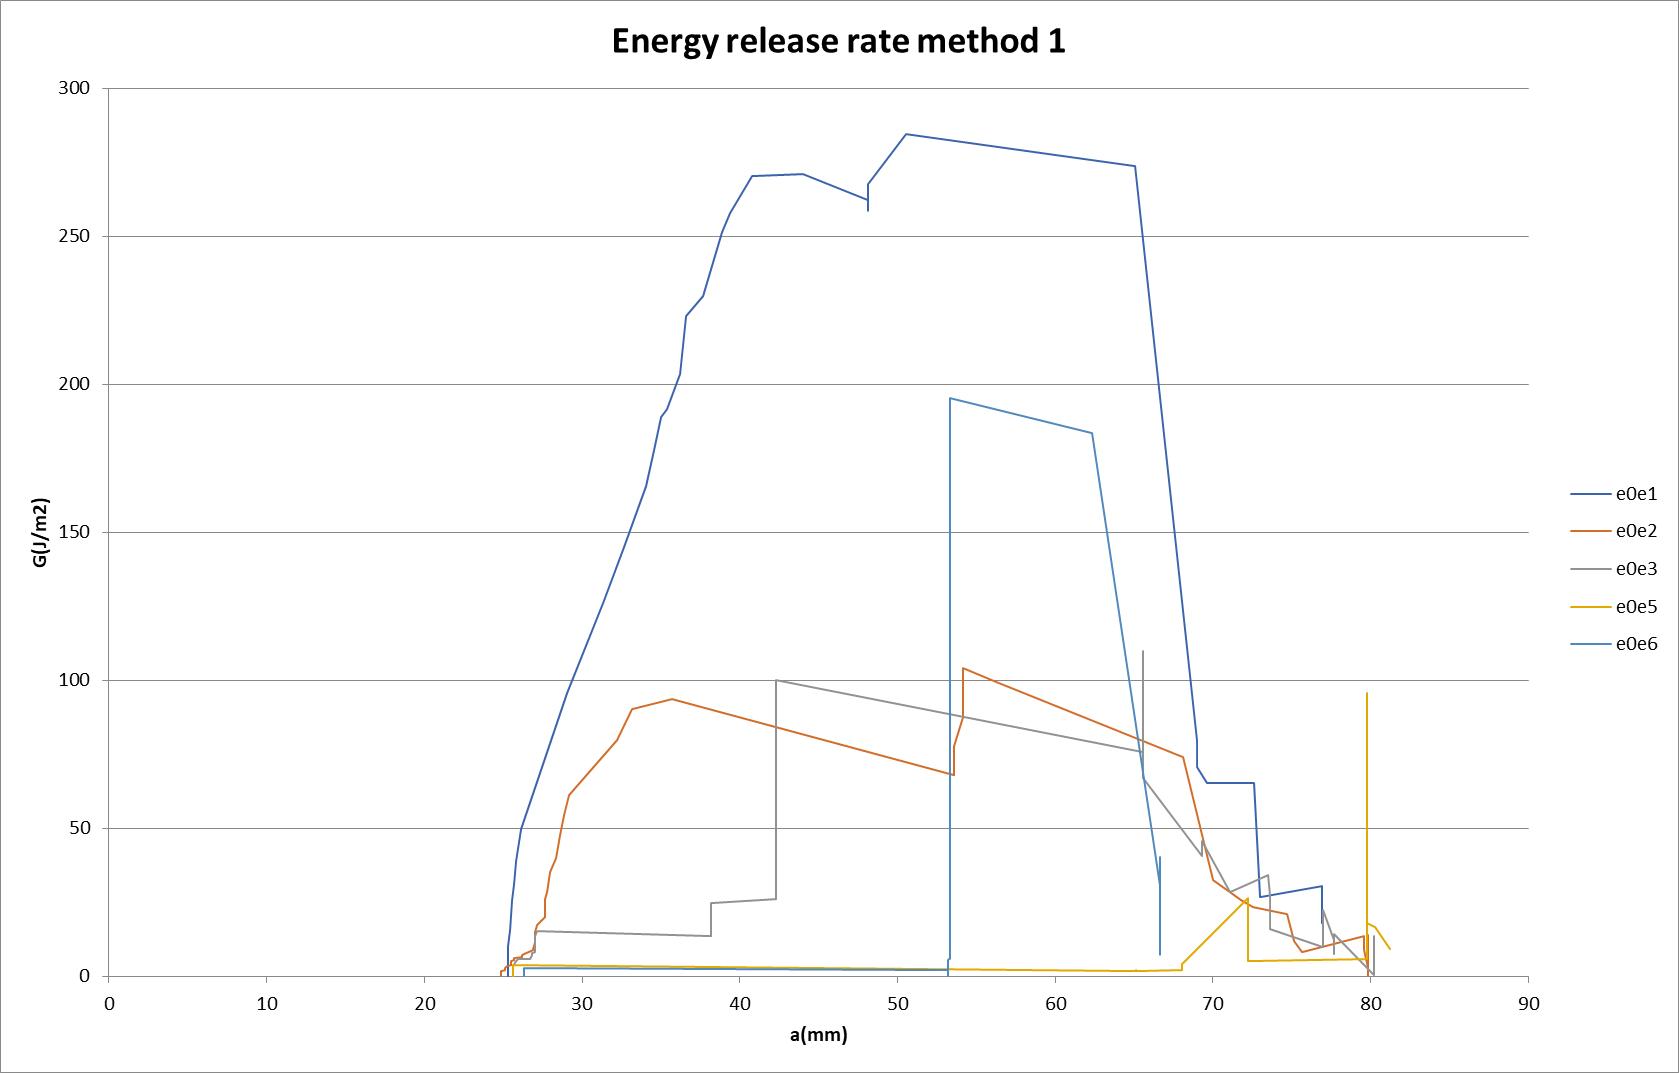
\includegraphics[width=13cm]{G_method1}
	\caption{$G$ obtaiend from method 1.}
	\label{fig:G_method1}
\end{figure}

\begin{figure}[htp]
	\centering
	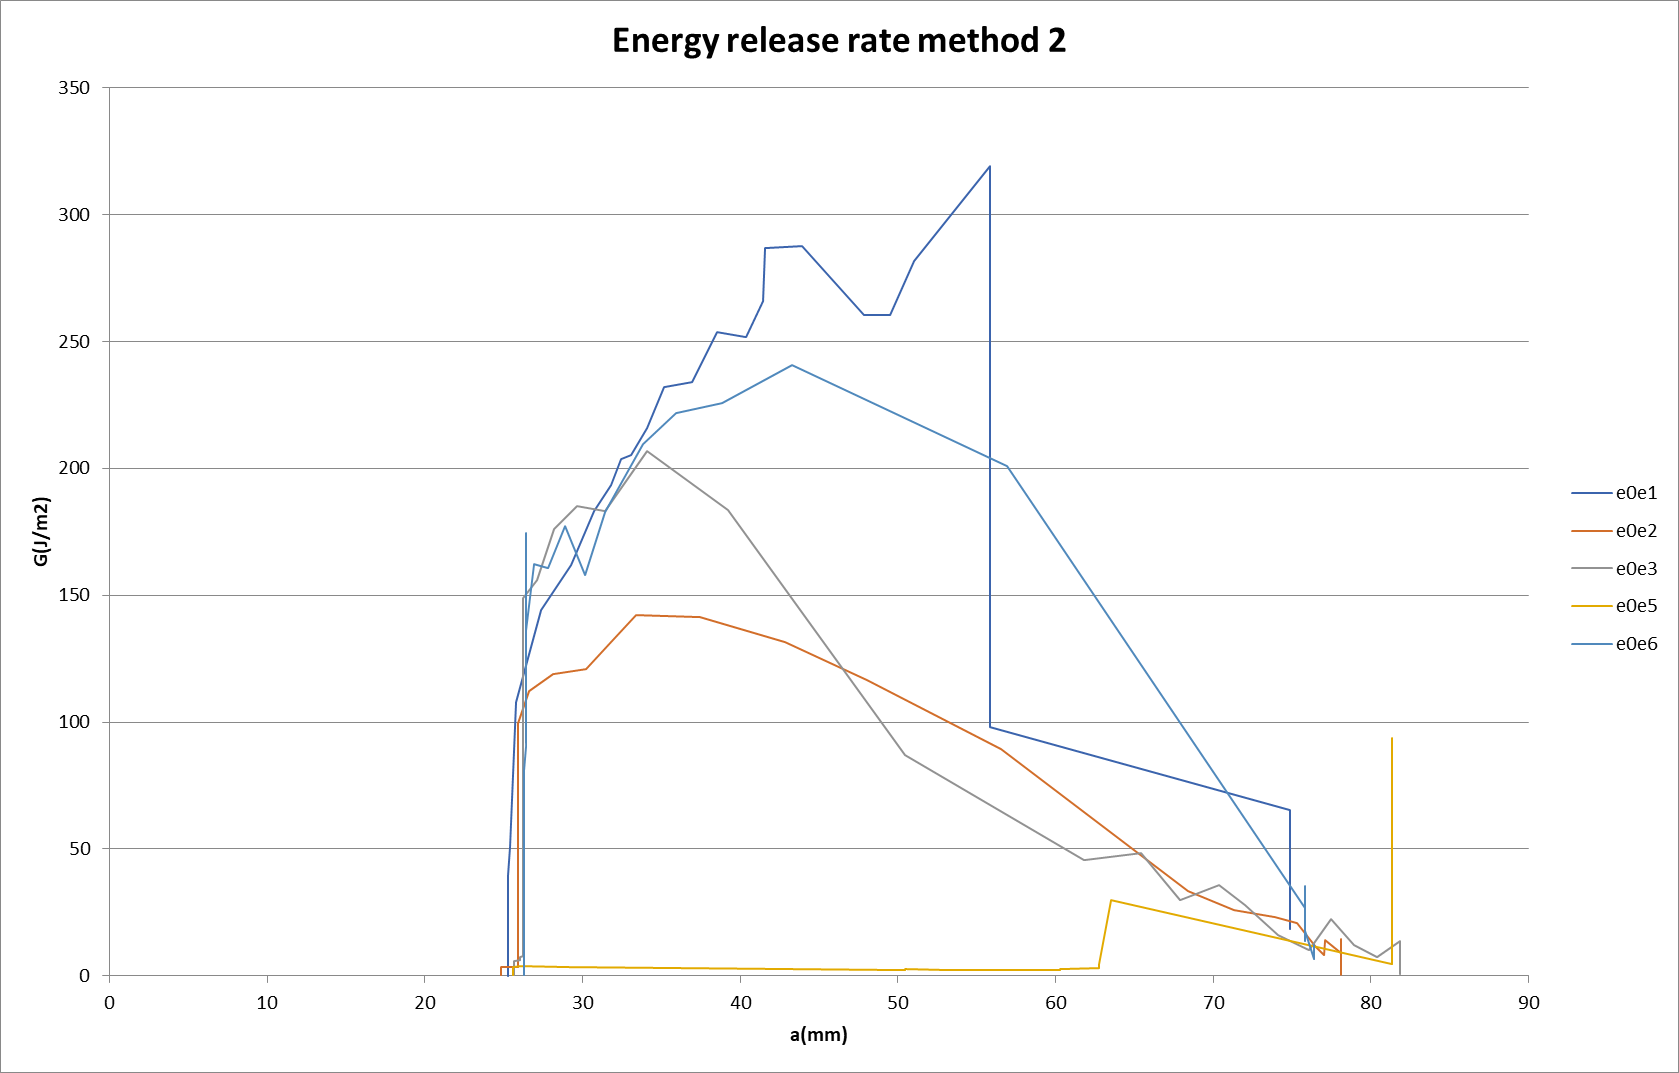
\includegraphics[width=13cm]{G_method2}
	\caption{$G$ obtaiend from method 2.}
	\label{fig:G_method2}
\end{figure}

We notice that G increases progressively with method 1 and Figure \ref{fig:G_method1} looks like the plots of G obtained by \cite{Odounga2018phd}. For method 2, it seems that G grows faster for a smaller increase in a(t). Indeed, for the same training period a(t) is generally higher with method 1 than with method 2. This proves that a slight variation in the crack length measurement produces completely different results for G. We can also see that the plots generally reach a plateau, which is the expected shape for the curve.
The figures of G can be seen one by one in appendix \ref{Appendix1}. This makes it easier to see the shape of the curve for each specimen.

Table \ref{fig:tableG1} gives the maximum values of G in mode I for silver Fir. It can be seen that G tends to be higher using method 2, which can be explained by a lower estimate of a(t) for the same image/stage.

\begin{table} [H]
	\centering
	\begin{tabular}{ccccccc}
		\toprule % horizontal line at the top of the table
		&  & e0e1 & e0e2 & e0e3 & e0e5 & e0e6\\\midrule
		& Gmax method1, ($J/m^2$) & 284.44 & 90.24 & 107.49 & 95.67 & 183.58 \\\midrule
		& Gmax method2, ($J/m^2$) & 286.65 & 131.16 & 206.73 & 93.83 & 199.59 \\\midrule
	\end{tabular}
	\caption{$G_\text{Imax}$ values for Silver Fir specimens in mode I.}
	\label{fig:tableG1}
\end{table}

\subsection{Discussion}

Table \ref{fig:fig37} compares the different values of the maximum energy release rate obtained in this study with the literature review. These are numerous, especially in mode I. In order to provide an objective comparison, the discussion focuses on temperate species with a similar density, a moisture content between 9\% and 12\% and an initial crack oriented in the RL direction. The average maximum energy release rate for silver fir is shown in bold and compared to different species and different tests. There are 2MCG, DCB and Wedge Splitting tests.
First of all, we can see that the value of G is of the same order of magnitude as for the other species. Silver fir differs from alder by $29 \%$, pinus pinaster by $36 \%$ and Padouk by $33 \%$. Moreover, in \cite{Odounga2018phd}'s work it's not uncommon to obtain similar values. In fact, his standard deviation is 2 to 3 times greater, which means that his results are more widely dispersed.
\cite{Xavieretal2014} also obtained experimental values of G=190 J/m2, which corresponds to the results obtained in this study. In addition, alder and pinus pinaster are not very far from silver fir in density (around 0.1).
The scattering of results observed here can be attributed to the material. This dispersal is justified by the high natural variability of wood and its anatomical composition.
In addition, different methods have been used to measure the energy release rate and the use of various experimental parameters inevitably impacts the final results.
On the other hand, it seems that the specimens were created more with the extremity of the tree trunk than with its centre. We can see that there is a certain inclination of the tree rings when we look at our specimens. This could explain the slightly lower value obtained by our tests since $G_{RL}> G_{TL}$ as shown in the article by \cite{Reiterer2002}.

\begin{table}[H]
	\centering
	\resizebox{\textwidth}{!}{
		\begin{tabular}{cccccccc}
			\toprule % ligne horizontale en haut du tableau
			& References & Wood species & Test type & Orientation & Density & $G_{\max}(J/m^2)$ & Standard deviation \\
			\midrule
			& & \textbf{Silver fir} & \textbf{2MCG} & \textbf{RL} & \textbf{0.43} & \textbf{170} & \textbf{77} \\
			\midrule
			& \cite{Angellier2017} & Douglas fir & DCB & RL & 0.54 & 784 &  \\
			\midrule
			& \cite{Angellier2017} & White fir & DCB & RL & 0.49 & 570 &  \\
			\midrule
			& \cite{Xavieretal2014} & Pinus Pinaster & DCB & RL & 0.543 & 270 & 64 \\
			\midrule
			& \cite{Reiterer2002} & Spruce & WS & RL & 0.479 & 337 & 47 \\
			\midrule
			& \cite{Reiterer2002} & Alder & WS & RL & 0.510 & 244 & 41 \\
			\midrule
			& \cite{Reiterer2002} & Oak & WS & RL & 0.553 & 348 & 38 \\
			\midrule
			& \cite{Reiterer2002} & Ash & WS & RL & 0.701 & 551 & 38 \\
			\midrule
			& \cite{Odounga2018phd} & Okoumé & 2MCG & RL & 0.39-0.5 & 317 & 160 \\
			\midrule
			& \cite{Odounga2018phd} & Iroko & 2MCG & RL & 0.56-0.7 & 323 & 200 \\
			\midrule
			& \cite{Odounga2018phd} & Padouk & 2MCG & RL & 0.7-0.88 & 255 & 200 \\
			\bottomrule % ligne horizontale en bas du tableau
		\end{tabular}
	}
	\caption{Comparison of mean max G values for specimens in the literature, 2MCG: Mixed Mode Crack Growth, DCB: Double Cantilever Beam, WS: Wedge Splitting test, RL: Radial Longitudinal.}
	\label{fig:fig37}
\end{table}


\section{Conclusion}

In this study, cracking tests were carried out on a softwood, Silver Fir. A speckle pattern was transferred to each specimen to follow the progress of the crack front and measure its opening. Two methods were used and compared to measure the crack front. It seems that method 1 is more effective than method 2. The variables obtained from the DIC method were used to calculate the critical energy release rate for each specimen using the compliance method. Comparison of the Gmax averages with those for temperate species given in the literature review shows that the results obtained are similar, although slightly lower. 